\documentclass{standalone}
\usepackage{tikz}
\usetikzlibrary{arrows.meta}

\begin{document}

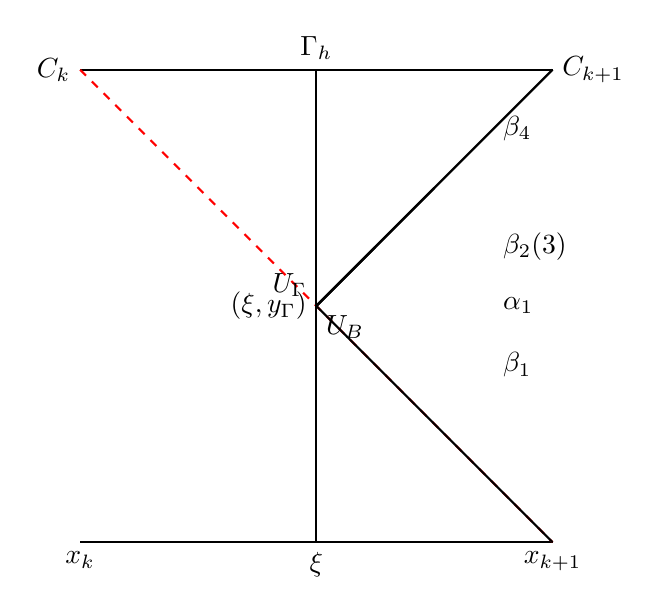
\begin{tikzpicture}[scale=1.5]
    % Draw the vertical lines
    \draw[thick] (0,0) -- (4,0);
    \draw[thick] (0,4) -- (4,4);
    
    % Label the points
    \node at (0,4) [left] {$C_k$};
    \node at (4,4) [right] {$C_{k+1}$};
    \node at (0,0) [below] {$x_k$};
    \node at (4,0) [below] {$x_{k+1}$};
    \node at (2,0) [below] {$\xi$};
    \node at (2,4) [above] {$\Gamma_h$};
    
    % Draw the red line
    \draw[red, thick, dashed] (0,4) -- (4,0);
    
    % Draw the horizontal lines
    \draw[thick] (2,0) -- (2,4);
    
    % Label the intersection point
    \node at (2,2) [left] {$(\xi, y_\Gamma)$};
    
    % Draw the diagonal lines
    \draw[thick] (2,2) -- (4,4);
    \draw[thick] (2,2) -- (4,0);
    \draw[thick] (2,2) -- (3,3);
    \draw[thick] (2,2) -- (2.5,2.5);
    
    % Label the angles
    \node at (3.5,3.5) [right] {$\beta_4$};
    \node at (3.5,2.5) [right] {$\beta_2(3)$};
    \node at (3.5,2) [right] {$\alpha_1$};
    \node at (3.5,1.5) [right] {$\beta_1$};
    
    % Draw the labels for the regions
    \node at (2,2) [below right] {$U_B$};
    \node at (2,2) [above left] {$U_\Gamma$};
\end{tikzpicture}

\end{document}